\subsection{Struktur der Proben}

Alle in diesem Versuch untersuchten Materialien (Gold und Graphit) sind Leiter. Sie unterscheiden sich jedoch in der Elektronenkonfiguration. Es gibt einen Unterschied zwischen der Verteilung der Elektronen in Metallen und Halbleitern. Die Elektronen von Metallen und Halbleitern k�nnen im periodischen Potential der Atomr�mpfe z.B. mit der Schr�dingergleichung und einigen Annahmen analysiert werden. Es stellt sich heraus, dass sogenannte verbotene Zonen (Bandl�cken) entstehen. Die Energieniveas, die mit Elektronen besetzt werden k�nnen, werden B�nder bezeichnet. Bei Metallen ist das oberste Band nicht voll besetzt, sodass sich Elektronen frei in dem Band bewegen k�nnen. Bei Halbleitern ist das oberste Band voll, sodass erst durch z.B. thermische Anregung Elektronen in ein h�heres Band (Leitungsband) angeregt werden k�nnen, in welchem sie sich dann ebenfalls frei bewegen k�nnen. Das oberste nicht voll besetzte Band wird Leitungsband genannt. Es soll nun genauer auf die beiden bekannten Proben Gold und Graphit eingegangen werden.

\subsubsection{Graphit}

Die Graphitprobe ist ein HOPG (highly orderd pyrolytic graphit), ein Halbleiter mit einer hcp-Gitterstruktur. In Abbildung \ref{fig:graphit} ist die Gitterstruktur des Graphits zu sehen. In einer Ebene werden die Kohlenstoffatome aufgrund der sp2-Hybirdisirung  stark durch kovalente Bindungen zusammengehalten. Zwischen den Ebenen werden die Kohlenstoffatome nur von Van-der-Waals-Kr�ften zusammengehalten. 

\begin{figure}[H]
	\centering
  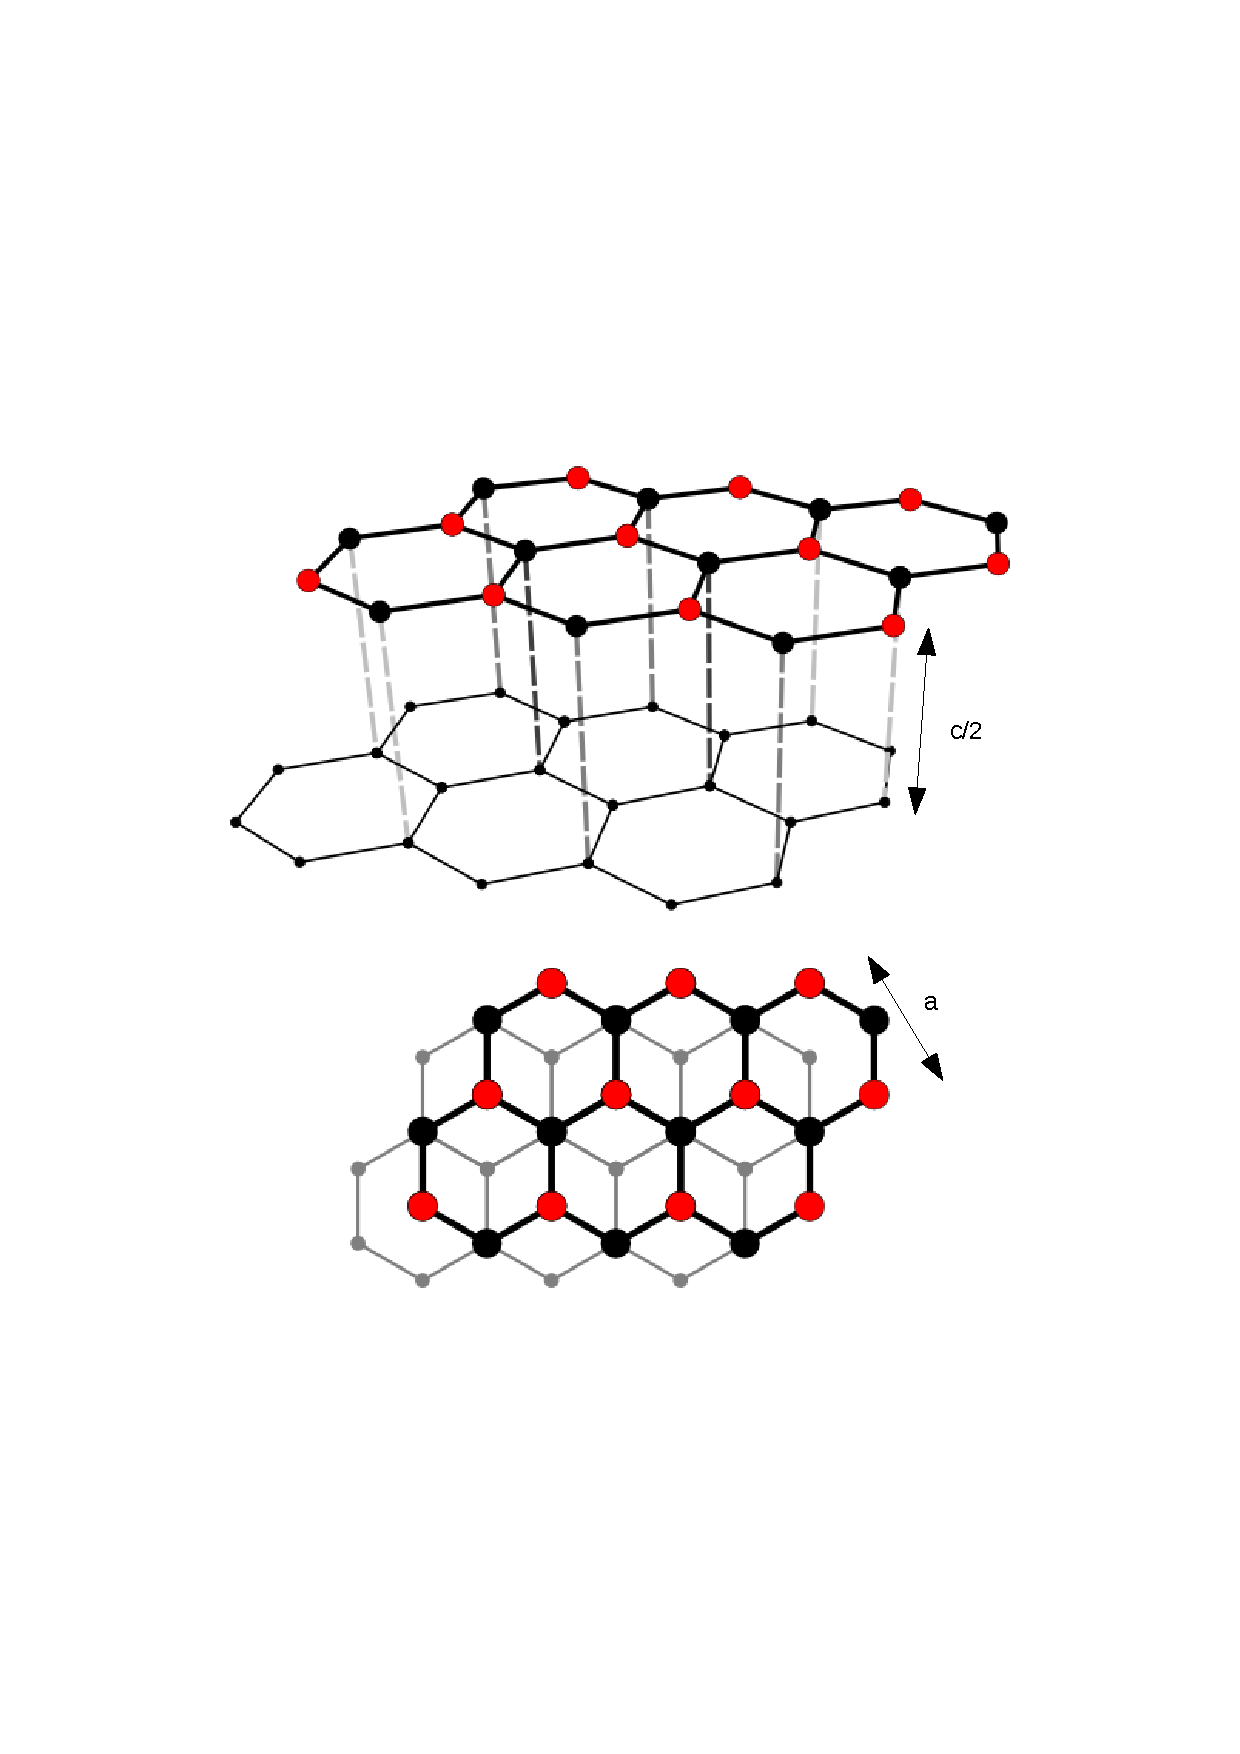
\includegraphics[trim = 10mm 70mm 30mm 60mm, clip,scale=0.8]{graphit.pdf}
	\caption{Schematische Struktur von Graphit. Die Ebenen liegen in ABAB-Form vor, sodass jede zweite Ebene gleich aufliegt. Die Ebenen untereinander besitzen an jeder zweiten Ecke des Hexagons eine Verbindung. Entnommen von \cite{graphit-bild}, modifiziert}
	\label{fig:graphit}
\end{figure}

Die in Abbildung \ref{fig:graphit} eingezeichneten Gitterkonstanten haben die Werte a = \SI{2,46}{\angstrom} und c = \SI{6,71}{\angstrom} (vgl. \cite{graphit}). Aufgrund ABAB-Form liegen immer drei Atome in den Hexagonalen etwas erh�ht und haben so eine h�here frei elektrische Zustandsdichte. Diese Struktur ist mit dem RTM zu sehen.

\subsubsection{Gold}
Gold hat eine fcc-Kristallstruktur. Die Gitterkonstante betr�gt a = \SI{4.065}{\angstrom}  \cite{PhysRev.25.753}. Untersucht wird die (111)-Goldschicht, wobei (111) die Millerindizes sind, die die Struktur der betrachteten Ebene des Kristalls beschreiben. Die atomare Struktur von Gold ist deutlich schwerer zu messen, da die Atome homogen verteilt sind.